\section{Magnetic order and spin waves}\label{sec:7.1}

Each nickel ion in NiO carries a spin, and below \SI{523}{K}, the measured Néel temperature~\cite[Table~IV]{fischer2009exchange}, the spins order: those in one $(111)$ plane of the crystal point one way, those in the next plane the opposite way. A disturbance of that order travels through the crystal as a spin wave. The quanta of spin waves, the \emph{magnons}, have energies up to ${\sim}\SI{117}{meV}$. Inelastic neutron scattering at \SI{78}{K} measured their dispersion, with an initial slope of ${\sim}\SI{250}{meV.\angstrom}$~\cite{hutchings1972measurement}. In an ordered magnet a particle that couples to the spin of the electron can create a magnon~\cite{trickle2020detecting}. The energy deposits then run from a few meV to about a tenth of an eV. To compute the rate of magnon creation we need the interaction that orders the spins, the spectrum of the spin waves, and the operator through which a probe creates magnons.

\subsection{Exchange and the Heisenberg model}

The Coulomb interaction does not act on spin, yet it makes the energy of two electrons depend on how their spins are aligned. Put one electron in each of two orthogonal orbitals $\varphi_a$ and $\varphi_b$. In the spin triplet the spatial wavefunction is antisymmetric, $[\varphi_a(\vect{r})\varphi_b(\vect{r}') - \varphi_b(\vect{r})\varphi_a(\vect{r}')]/\sqrt2$, and in the singlet it is symmetric. The expectation value of the Coulomb repulsion $v_{\mathrm{C}}(\vect{r} - \vect{r}')$ is then $C \mp K_{\mathrm{ex}}$, upper sign for the triplet, with the direct integral $C$ and the exchange integral
\begin{equation}
  K_{\mathrm{ex}} = \int\dd^3r\,\dd^3r'\,\varphi_a^*(\vect{r})\varphi_b^*(\vect{r}')\,v_{\mathrm{C}}(\vect{r} - \vect{r}')\,\varphi_b(\vect{r})\varphi_a(\vect{r}') .
  \label{eq:7.1-Kex}
\end{equation}
The exchange integral $K_{\mathrm{ex}}$ is the exchange term of \cref{eq:2.3-direct-exchange}, written for localized orbitals instead of plane waves. It is the Coulomb self-energy of the charge distribution $\varphi_a^*\varphi_b$, and since the Fourier transform $v_{\mathrm{C}}(k) = e^2/k^2$ is positive, $K_{\mathrm{ex}} > 0$. The triplet therefore lies $2K_{\mathrm{ex}}$ below the singlet: parallel spins keep the electrons apart and save Coulomb energy. The resulting preference for parallel spins is Hund's rule, and within one Ni$^{2+}$ ion it aligns the two holes of the $3d$ shell into a spin $|\vect{S}| = 1$.

The four spin states can be described without any reference to orbitals. With $\vect{S}_1\cdot\vect{S}_2 = \frac12[(\vect{S}_1 + \vect{S}_2)^2 - \vect{S}_1^2 - \vect{S}_2^2]$, which is $-\frac34$ in the singlet and $\frac14$ in the triplet, the operator
\begin{equation}
  H_{12} = E_{\mathrm{orb}} + C - \tfrac12K_{\mathrm{ex}} - 2K_{\mathrm{ex}}\,\vect{S}_1\cdot\vect{S}_2
  \label{eq:7.1-dirac}
\end{equation}
has the singlet energy $E_{\mathrm{orb}} + C + K_{\mathrm{ex}}$ and the triplet energy $E_{\mathrm{orb}} + C - K_{\mathrm{ex}}$, with $E_{\mathrm{orb}}$ the sum of the two one-electron orbital energies. The Coulomb interaction depends only on the positions of the electrons, and through exchange it has become a coupling between their spins, of strength $-2K_{\mathrm{ex}}$ and ferromagnetic sign.

\paragraph{Kinetic exchange.} Between electrons on neighboring ions of an insulator, however, a second mechanism usually dominates, and it has the opposite sign. Take two sites with one orbital each and the hopping $t_{\mathrm{hop}} > 0$ of the tight-binding model of \cref{sec:3.2}. Putting two electrons on the same site costs the on-site or Hubbard repulsion $U_{\mathrm{H}}$:
\begin{equation}
  H = -t_{\mathrm{hop}}\sum_{s}\bigl(c^\dagger_{1s}c_{2s} + c^\dagger_{2s}c_{1s}\bigr) + U_{\mathrm{H}}\sum_{i=1,2}c^\dagger_{i\uparrow}c_{i\uparrow}\,c^\dagger_{i\downarrow}c_{i\downarrow} .
  \label{eq:7.1-hubbard}
\end{equation}
With two electrons and $t_{\mathrm{hop}} = 0$, the four states with one electron on each site are degenerate at zero energy, and the two doubly occupied states lie at $U_{\mathrm{H}}$. The hopping connects the singly occupied states with the doubly occupied ones. A triplet cannot hop, since the Pauli principle forbids two parallel spins in one orbital: for the state $c^\dagger_{1\uparrow}c^\dagger_{2\uparrow}|0\rangle$ the hop is blocked directly, and the other two members of the triplet follow by rotational symmetry. The triplet stays at zero energy to all orders. The singlet couples to the symmetric combination of the doubly occupied states, through two hops (from site 1 or from site 2) that add, with a matrix element of magnitude $2t_{\mathrm{hop}}$. To second order in $t_{\mathrm{hop}}/U_{\mathrm{H}}$ its energy is $-(2t_{\mathrm{hop}})^2/U_{\mathrm{H}}$. As \cref{eq:7.1-dirac} shows, the coefficient of $\vect{S}_1\cdot\vect{S}_2$ is the triplet energy minus the singlet energy. With both mechanisms present the coefficient is
\begin{equation}
  J^{\mathrm{ex}} = \frac{4t_{\mathrm{hop}}^2}{U_{\mathrm{H}}} - 2K_{\mathrm{ex}} .
  \label{eq:7.1-superexchange}
\end{equation}
The picture behind the first term is that an electron lowers its kinetic energy by a virtual hop onto its neighbor and back, and it can do so only if the neighbor's spin is antiparallel. The virtual hop costs $U_{\mathrm{H}}$, so the kinetic-energy gain is second order in $t_{\mathrm{hop}}$. The second-order expansion holds as long as $t_{\mathrm{hop}} \ll U_{\mathrm{H}}$. The same condition keeps the charge frozen at one electron per site, and in this two-site picture an insulator with frozen charge of this kind is a \emph{Mott insulator}. The corrections to \cref{eq:7.1-superexchange} are of relative order $(t_{\mathrm{hop}}/U_{\mathrm{H}})^2$.

In NiO the nickel ions do not touch; between two of them sits an oxygen ion. Anderson's mechanism of \emph{superexchange}~\cite{anderson1959new} applies \cref{eq:7.1-superexchange} with an effective hopping that runs through the oxygen $p$ orbital, so that $t_{\mathrm{hop}}$ is itself second order in the nickel--oxygen hopping. The geometry of the nickel--oxygen--nickel bond then decides the sign and the size of the coupling. Next-nearest nickel neighbors sit on a straight line through one oxygen ion. The oxygen $p$ orbital along that line overlaps strongly with a $3d$ orbital of each nickel ion, and the coupling of next-nearest neighbors is large and antiferromagnetic. Nearest neighbors see each other at \ang{90} through two different $p$ orbitals, and their coupling is weak and ferromagnetic. The measured values are~\cite{hutchings1972measurement}
\begin{equation}
  J_2 = \SI{19.01}{meV}, \qquad J_1 = -\SI{1.37}{meV} ,
  \label{eq:7.1-NiO}
\end{equation}
in the convention of \cref{eq:7.1-heis} below. With several $3d$ orbitals and $|\vect{S}| = 1$, \cref{eq:7.1-superexchange} acquires factors of order one, and we use it as an estimate, $J^{\mathrm{ex}} \sim t_{\mathrm{hop}}^2/U_{\mathrm{H}}$. The Hubbard repulsion of the nickel $3d$ shell is several eV; the linear-response values of \cref{app:E.9} lie between 4.6 and \SI{8.2}{eV}. Inverting the estimate for $J_2$ gives an effective hopping $(J_2U_{\mathrm{H}})^{1/2} \approx 0.3$ to \SI{0.4}{eV}, so that $t_{\mathrm{hop}}/U_{\mathrm{H}} \approx 0.05$ to 0.06. Since the electrons of NiO hop little compared with the cost of a double occupancy, only their spins remain free at low energy. The estimate is rough in one more respect. NiO is a \emph{charge-transfer insulator}: the cheapest charge excitation moves an electron from oxygen to nickel, at the charge-transfer energy $\Delta_{\mathrm{CT}}$, which is smaller than $U_{\mathrm{H}}$. Superexchange through the oxygen depends on both $\Delta_{\mathrm{CT}}$ and $U_{\mathrm{H}}$, and the effective hopping above absorbs the two energies into one number.

\paragraph{The Heisenberg model.} In a crystal of ions with frozen charge, each carrying a spin of length $|\vect{S}|$ fixed by Hund's rule, the low-energy states are the spin configurations. To leading order in $t_{\mathrm{hop}}/U_{\mathrm{H}}$ the coupling of the spins is a sum over pairs, and the only coupling of two spins that is invariant under a common rotation and bilinear in each is their scalar product. The result is the \emph{Heisenberg model},
\begin{equation}
  H_{\mathrm{H}} = \sum_{\langle ij\rangle}J^{\mathrm{ex}}_{ij}\,\vect{S}_i\cdot\vect{S}_j ,
  \label{eq:7.1-heis}
\end{equation}
with each pair of ions counted once and the \emph{exchange constant} $J^{\mathrm{ex}}_{ij} > 0$ antiferromagnetic. The ionic spins obey $[S^a_i, S^b_j] = \ii\delta_{ij}\epsilon_{abc}S^c_i$ and $\vect{S}_i^2 = |\vect{S}|(|\vect{S}| + 1)$. The literature uses every combination of sign, of single or double counting and of spin length, and a quoted $J^{\mathrm{ex}}$ is meaningful only together with its Hamiltonian.

If every $J^{\mathrm{ex}}_{ij} < 0$, the ground state has all spins parallel, and the magnet is a \emph{ferromagnet}. If the antiferromagnetic bonds connect two sublattices, the classical ground state has the spins of one sublattice up and those of the other down, and the magnet is an \emph{antiferromagnet}. In NiO, $J_2$ connects the ions of adjacent $(111)$ planes, and the order is the alternation of ferromagnetic $(111)$ planes described above, called type~II (\cref{fig:7-nio}a). \Cref{eq:7.1-heis} leaves out the coupling of the spins to the lattice through spin--orbit coupling. The spin--orbit coupling fixes the direction of the moments in the crystal and opens small gaps in the magnon spectrum, below \SI{5}{meV} in NiO~\cite[Sect.~III]{dossantos2026comparative}, and we neglect it.

The exchange constants of a real magnet are computed from the electronic structure. The standard method is the density-functional theory (DFT) of \cref{sec:3.4} with a Hubbard correction on the $3d$ shell, called DFT~$+\,U$. Three routes are common: total energies of several collinear orders mapped onto \cref{eq:7.1-heis}, the energies of spin spirals, and a Green's-function formula for small rotations of two moments. All three inherit the dependence of superexchange on $U_{\mathrm{H}}$. For NiO the density-functional values of $J_2$ in one comparison range from 11 to \SI{27}{meV}~\cite[Table~III]{fischer2009exchange}, and linear spin-wave theory with the best of them overestimates the measured maximum magnon energy by about \SI{14}{\percent}~\cite[Sect.~III]{dossantos2026comparative}. For a target without neutron data, this spread is the theory uncertainty of its magnon spectrum.

\subsection{Spin waves of a ferromagnet}

The ferromagnetic ground state is known exactly, and its excitations are the simplest place to see what a magnon is. Order the spins along $+\hat{\vect{z}}$. Removing one unit of spin from site $j$ does not give an eigenstate, because the transverse part of $\vect{S}_i\cdot\vect{S}_j = S^z_iS^z_j + \frac12(S^+_iS^-_j + S^-_iS^+_j)$ moves this spin deviation to the neighbors. The eigenstates, the spin waves, are spin deviations spread over all sites with a definite crystal momentum.

Holstein and Primakoff turned this into a boson problem~\cite{holstein1940field}. On each site write
\begin{equation}
  S^z_j = |\vect{S}| - d^\dagger_jd_j, \qquad
  S^+_j = \bigl(2|\vect{S}| - d^\dagger_jd_j\bigr)^{1/2}d_j, \qquad
  S^-_j = d^\dagger_j\bigl(2|\vect{S}| - d^\dagger_jd_j\bigr)^{1/2} ,
  \label{eq:7.1-HP}
\end{equation}
with boson operators $[d_i, d^\dagger_j] = \delta_{ij}$ of the kind introduced in \cref{sec:2.3}. The number $n_j = d^\dagger_jd_j$ counts the deviation of the site from full polarization. The spin algebra holds on the physical states $n_j \le 2|\vect{S}|$. To check $[S^+, S^-] = 2S^z$ on one site, use $f(n)d = d\,f(n - 1)$ for any function $f$. Then $S^+S^- = (2|\vect{S}| - n)(n + 1)$ and $S^-S^+ = d^\dagger(2|\vect{S}| - n)d = n(2|\vect{S}| - n + 1)$, and the difference of the two products is $2|\vect{S}| - 2n = 2S^z$; the relations $[S^z, S^\pm] = \pm S^\pm$ follow since $S^+$ lowers $n$ by one. The square roots make \cref{eq:7.1-HP} exact and nonlinear. \emph{Linear spin-wave theory} is an expansion in $1/|\vect{S}|$, valid when the number of deviations per site is small compared with $2|\vect{S}|$. It replaces the square roots by $(2|\vect{S}|)^{1/2}$ and keeps the Hamiltonian to second order in the bosons. For one bond,
\begin{equation*}
  \vect{S}_i\cdot\vect{S}_j \simeq |\vect{S}|^2 - |\vect{S}|\bigl(n_i + n_j\bigr) + |\vect{S}|\bigl(d^\dagger_id_j + d^\dagger_jd_i\bigr) ,
\end{equation*}
where the dropped quartic term $n_in_j$ comes from $S^z_iS^z_j$. The deviations hop from site to site with amplitude $J^{\mathrm{ex}}_{ij}|\vect{S}|$.

On a Bravais lattice of $N$ magnetic ions at the sites $\vect{R}_j$, the hopping is diagonalized by plane waves,
\begin{equation*}
  d_j = N^{-1/2}\sum_{\vect{k}}\ee^{\ii\vect{k}\cdot\vect{R}_j}\,a_{\vect{k}} ,
\end{equation*}
with $\vect{k}$ in the Brillouin zone. The operators $a_{\vect{k}}$ are bosons, the \emph{magnon operators}; with several magnetic ions per cell they carry a branch index, $a_{\vect{k}\nu}$, which we drop for a single branch. In the sum over pairs, each site has the bonds $\sum_{\vect{R}\neq0}J^{\mathrm{ex}}_{0\vect{R}}$, which multiply $-|\vect{S}|n_j$, and the hopping terms collect into $|\vect{S}|\sum_{\vect{k}}J^{\mathrm{ex}}(\vect{k})\,a^\dagger_{\vect{k}}a_{\vect{k}}$ with the lattice Fourier transform of the exchange constants. The result is a set of independent oscillators:
\begin{keyresult}[Linear spin waves of a ferromagnet]
\begin{equation}
  H_{\mathrm{H}} \simeq E_{\mathrm{cl}} + \sum_{\vect{k}}\omega^{\mathrm{M}}_{\vect{k}}\,a^\dagger_{\vect{k}}a_{\vect{k}}, \qquad
  \omega^{\mathrm{M}}_{\vect{k}} = |\vect{S}|\bigl[J^{\mathrm{ex}}(\vect{k}) - J^{\mathrm{ex}}(0)\bigr], \qquad
  J^{\mathrm{ex}}(\vect{k}) = \sum_{\vect{R}\neq0}J^{\mathrm{ex}}_{0\vect{R}}\,\ee^{\ii\vect{k}\cdot\vect{R}} ,
  \label{eq:7.1-fm}
\end{equation}
with the classical energy $E_{\mathrm{cl}} = \frac12N|\vect{S}|^2J^{\mathrm{ex}}(0)$, each pair counted once.
\end{keyresult}
For inversion-symmetric lattices $J^{\mathrm{ex}}(\vect{k})$ is real and even. With all $J^{\mathrm{ex}}_{0\vect{R}} < 0$, $J^{\mathrm{ex}}(0)$ is the minimum of $J^{\mathrm{ex}}(\vect{k})$ and every $\omega^{\mathrm{M}}_{\vect{k}} \ge 0$. The mode $\omega^{\mathrm{M}}_0 = 0$ tilts all spins together. A common tilt costs nothing because \cref{eq:7.1-heis} is invariant under a common rotation, and the mode $\omega^{\mathrm{M}}_0 = 0$ is the Goldstone mode of the broken rotational symmetry, the analog of the acoustic phonon of a crystal. A particle physicist would count two Goldstone modes for the two broken rotations about $\hat{\vect{x}}$ and $\hat{\vect{y}}$. The ferromagnet has one, with a quadratic dispersion. Its two broken generators do not commute in the ground state, $\langle[S^x_{\mathrm{tot}}, S^y_{\mathrm{tot}}]\rangle = \ii\langle S^z_{\mathrm{tot}}\rangle \ne 0$, so they act as a coordinate and its conjugate momentum and together describe a single mode. In the antiferromagnet $\langle S^z_{\mathrm{tot}}\rangle = 0$, and the two Goldstone modes of the particle physicist's count appear, both with a linear dispersion. At small $k$, expanding $J^{\mathrm{ex}}(\vect{k})$ to second order gives $\omega^{\mathrm{M}}_{\vect{k}} \simeq \frac12|\vect{S}|\sum_{\vect{R}}(-J^{\mathrm{ex}}_{0\vect{R}})(\vect{k}\cdot\vect{R})^2$, quadratic in $k$ like the energy of a free particle. Physically, the magnon $a^\dagger_{\vect{k}}|0\rangle$ is one unit of spin deviation shared by all ions: each spin precesses on a narrow cone about $\hat{\vect{z}}$, and the phase of the precession advances by $\vect{k}\cdot\vect{R}$ from ion to ion.

\begin{workedexample}{The ferromagnetic chain}\label{we:7-chain}
Take a ring of $N$ spins at spacing $a$ with ferromagnetic nearest-neighbor exchange $J^{\mathrm{ex}} < 0$. Then $J^{\mathrm{ex}}(k) = 2J^{\mathrm{ex}}\cos ka$, and \cref{eq:7.1-fm} gives
\begin{equation*}
  \omega^{\mathrm{M}}_k = 2|J^{\mathrm{ex}}||\vect{S}|\,(1 - \cos ka) ,
\end{equation*}
which rises as $|J^{\mathrm{ex}}||\vect{S}|a^2k^2$ from $k = 0$ and reaches $4|J^{\mathrm{ex}}||\vect{S}|$ at the zone boundary $k = \pi/a$.

For one magnon this linear result is exact. Let $|F\rangle$ be the fully polarized state, of energy $E_F = NJ^{\mathrm{ex}}|\vect{S}|^2$, and $|j\rangle = (2|\vect{S}|)^{-1/2}S^-_j|F\rangle$ the normalized state with one unit of deviation on site $j$. The bonds that do not touch $j$ keep their energy $J^{\mathrm{ex}}|\vect{S}|^2$. The two bonds that do touch site $j$ have $S^zS^z = |\vect{S}|(|\vect{S}| - 1)$, and together they raise $\langle j|H_{\mathrm{H}}|j\rangle$ to $E_F - 2J^{\mathrm{ex}}|\vect{S}|$, above $E_F$ since $J^{\mathrm{ex}} < 0$. The transverse term $\frac12J^{\mathrm{ex}}S^+_jS^-_{j\pm1}$ moves the deviation to a neighbor with amplitude $\frac12J^{\mathrm{ex}}\cdot2|\vect{S}| = J^{\mathrm{ex}}|\vect{S}|$, since each of the two operators contributes $(2|\vect{S}|)^{1/2}$: $S^-_{j\pm1}$ acting on a full site and $S^+_j$ acting on a site with one deviation. Hence
\begin{equation*}
  H_{\mathrm{H}}|j\rangle = (E_F - 2J^{\mathrm{ex}}|\vect{S}|)\,|j\rangle + J^{\mathrm{ex}}|\vect{S}|\,\bigl(|j + 1\rangle + |j - 1\rangle\bigr) ,
\end{equation*}
an exact statement for any $|\vect{S}|$, because the states with one deviation are closed under $H_{\mathrm{H}}$. The Bloch combination $N^{-1/2}\sum_j\ee^{\ii kja}|j\rangle$ is an eigenstate with energy $E_F - 2J^{\mathrm{ex}}|\vect{S}| + 2J^{\mathrm{ex}}|\vect{S}|\cos ka = E_F + \omega^{\mathrm{M}}_k$. The quartic terms dropped in linear spin-wave theory act only on states with two or more deviations, where they produce an attraction between magnons of relative order $1/|\vect{S}|$.

For dark matter the quadratic dispersion matters. A magnon of energy $\omega$ has $k = [\omega/(|J^{\mathrm{ex}}||\vect{S}|a^2)]^{1/2}$, and its group velocity $2(\omega|J^{\mathrm{ex}}||\vect{S}|)^{1/2}a$ vanishes at small $\omega$. At low energy a ferromagnet offers excitations of small momentum and small velocity, and their kinematic match differs from that of the linear branches of phonons and of the antiferromagnet below.
\end{workedexample}

\subsection{Spin waves of an antiferromagnet}\label{sec:7.1-afm}

In an antiferromagnet, however, the classical state with sublattice A up and sublattice B down is not an eigenstate of \cref{eq:7.1-heis}. For an antiparallel pair the transverse term $S^+_iS^-_j$, with $i$ on A and $j$ on B, lowers a spin that already points down and raises one that points up: it creates two deviations at once. This pair creation fixes the form of the antiferromagnetic spin waves. They are mixtures of deviations and their absence, and the Bogoliubov transformation of \cref{app:C.7} constructs them.

The magnetic ions form two interpenetrating sublattices A and B with $N_{\mathrm{s}}$ sites each, related by a translation or an inversion that exchanges them. On B the reference spin points along $-\hat{\vect{z}}$, so the roles of raising and lowering are exchanged: $S^z_j = -|\vect{S}| + d^\dagger_{\mathrm{B}j}d_{\mathrm{B}j}$ and $S^-_j \simeq (2|\vect{S}|)^{1/2}d_{\mathrm{B}j}$, while A uses \cref{eq:7.1-HP} with bosons $d_{\mathrm{A}i}$. At linear order an antiparallel bond becomes
\begin{equation*}
  \vect{S}_i\cdot\vect{S}_j \simeq -|\vect{S}|^2 + |\vect{S}|\bigl(n_{\mathrm{A}i} + n_{\mathrm{B}j}\bigr) + |\vect{S}|\bigl(d_{\mathrm{A}i}d_{\mathrm{B}j} + d^\dagger_{\mathrm{A}i}d^\dagger_{\mathrm{B}j}\bigr) ,
\end{equation*}
with $n_{\mathrm{A}i} = d^\dagger_{\mathrm{A}i}d_{\mathrm{A}i}$ and $n_{\mathrm{B}j}$ likewise. Each deviation raises the energy of the bond, and the pair term $d_{\mathrm{A}i}d_{\mathrm{B}j} + \text{h.c.}$ creates or destroys deviations in pairs. Bonds within a sublattice keep the ferromagnetic form. Exchange of any range enters through two lattice sums, over the neighbors of a site of A on its own sublattice and on the other,
\begin{equation}
  J^{\mathrm{ex}}_{\mathrm{AA}}(\vect{k}) = \sum_{\vect{\delta}\in\mathrm{A},\,\vect{\delta}\ne0}J^{\mathrm{ex}}_{0\vect{\delta}}\,\ee^{\ii\vect{k}\cdot\vect{\delta}}, \qquad
  J^{\mathrm{ex}}_{\mathrm{AB}}(\vect{k}) = \sum_{\vect{\delta}\in\mathrm{B}}J^{\mathrm{ex}}_{0\vect{\delta}}\,\ee^{\ii\vect{k}\cdot\vect{\delta}} ,
  \label{eq:D.19-Jk}
\end{equation}
where $\vect{\delta}$ runs over the positions of the neighbors relative to the site. The symmetry that exchanges A and B gives the same sums for a site of B. When the set of neighbors is symmetric under $\vect{\delta} \to -\vect{\delta}$, as it is for every lattice of this section, both $J^{\mathrm{ex}}_{\mathrm{AA}}(\vect{k})$ and $J^{\mathrm{ex}}_{\mathrm{AB}}(\vect{k})$ are real and even in $\vect{k}$.

Every site of A has the antiparallel bonds of total strength $J^{\mathrm{ex}}_{\mathrm{AB}}(0)$ and the parallel bonds $J^{\mathrm{ex}}_{\mathrm{AA}}(0)$, and likewise every site of B. Introduce
\begin{equation*}
  d_{\mathrm{A}i} = N_{\mathrm{s}}^{-1/2}\sum_{\vect{k}}\ee^{\ii\vect{k}\cdot\vect{R}_i}\,d_{\mathrm{A}\vect{k}}, \qquad
  d_{\mathrm{B}j} = N_{\mathrm{s}}^{-1/2}\sum_{\vect{k}}\ee^{-\ii\vect{k}\cdot\vect{R}_j}\,d_{\mathrm{B}\vect{k}} ,
\end{equation*}
with $\vect{k}$ in the Brillouin zone of one sublattice. The opposite sign on B is a convenience: $d_{\mathrm{B}\vect{k}}$ destroys a deviation of crystal momentum $-\vect{k}$, so that the pair terms couple $d_{\mathrm{A}\vect{k}}$ with $d_{\mathrm{B}\vect{k}}$. With $\sum_i\ee^{\ii(\vect{k}-\vect{k}')\cdot\vect{R}_i} = N_{\mathrm{s}}\delta_{\vect{k}\vect{k}'}$, the hopping terms on A give $|\vect{S}|\sum_{\vect{k}}J^{\mathrm{ex}}_{\mathrm{AA}}(\vect{k})\,d^\dagger_{\mathrm{A}\vect{k}}d_{\mathrm{A}\vect{k}}$, where each pair counted once contributes $J^{\mathrm{ex}}_{0\vect{\delta}}$ to both $\ee^{\ii\vect{k}\cdot\vect{\delta}}$ and $\ee^{-\ii\vect{k}\cdot\vect{\delta}}$. The hopping terms on B give the same with $\vect{k} \to -\vect{k}$, a substitution that changes nothing. The pair terms give $\sum_i\sum_{\vect{\delta}\in\mathrm{B}}J^{\mathrm{ex}}_{0\vect{\delta}}\,d_{\mathrm{A}i}d_{\mathrm{B},i+\vect{\delta}} = \sum_{\vect{k}}J^{\mathrm{ex}}_{\mathrm{AB}}(-\vect{k})\,d_{\mathrm{A}\vect{k}}d_{\mathrm{B}\vect{k}}$. Collecting all terms turns the Hamiltonian into a set of two-mode problems,
\begin{equation}
  \begin{gathered}
  H_{\mathrm{H}} \simeq E_{\mathrm{cl}} + |\vect{S}|\sum_{\vect{k}}\Bigl[A_{\vect{k}}\bigl(d^\dagger_{\mathrm{A}\vect{k}}d_{\mathrm{A}\vect{k}} + d^\dagger_{\mathrm{B}\vect{k}}d_{\mathrm{B}\vect{k}}\bigr) + B_{\vect{k}}\bigl(d_{\mathrm{A}\vect{k}}d_{\mathrm{B}\vect{k}} + d^\dagger_{\mathrm{B}\vect{k}}d^\dagger_{\mathrm{A}\vect{k}}\bigr)\Bigr] , \\
  A_{\vect{k}} = J^{\mathrm{ex}}_{\mathrm{AB}}(0) - J^{\mathrm{ex}}_{\mathrm{AA}}(0) + J^{\mathrm{ex}}_{\mathrm{AA}}(\vect{k}), \qquad B_{\vect{k}} = J^{\mathrm{ex}}_{\mathrm{AB}}(\vect{k}) .
  \end{gathered}
  \label{eq:7.1-Hk}
\end{equation}
The coefficient $A_{\vect{k}}$ is the cost of one deviation: the exchange field of the antiparallel neighbors minus that of the parallel ones, plus the hopping on its own sublattice. Without $B_{\vect{k}}$, \cref{eq:7.1-Hk} would describe a ferromagnet on each sublattice. At each $\vect{k}$, \cref{eq:7.1-Hk} is the two-mode Hamiltonian \cref{eq:C.7-Hboson}, with the diagonal energy $|\vect{S}|A_{\vect{k}}$ and the pairing amplitude $g_0 = |\vect{S}|B_{\vect{k}}$. The new operators
\begin{equation}
  a_{\vect{k}1} = u^{\mathrm{M}}_{\vect{k}}\,d_{\mathrm{A}\vect{k}} + v^{\mathrm{M}}_{\vect{k}}\,d^\dagger_{\mathrm{B}\vect{k}}, \qquad
  a_{\vect{k}2} = u^{\mathrm{M}}_{\vect{k}}\,d_{\mathrm{B}\vect{k}} + v^{\mathrm{M}}_{\vect{k}}\,d^\dagger_{\mathrm{A}\vect{k}} ,
  \label{eq:7.1-bogo}
\end{equation}
with $u^{\mathrm{M}}_{\vect{k}} = \cosh\theta_{\vect{k}}$ and $v^{\mathrm{M}}_{\vect{k}} = \sinh\theta_{\vect{k}}$, are bosons because $(u^{\mathrm{M}}_{\vect{k}})^2 - (v^{\mathrm{M}}_{\vect{k}})^2 = 1$, and the pair terms vanish for $\tanh2\theta_{\vect{k}} = B_{\vect{k}}/A_{\vect{k}}$. The coefficients $u^{\mathrm{M}}_{\vect{k}}$ and $v^{\mathrm{M}}_{\vect{k}}$ are the \emph{magnon Bogoliubov coefficients}. Equivalently,
\begin{equation*}
  (u^{\mathrm{M}}_{\vect{k}})^2 = \frac12\Bigl(\frac{A_{\vect{k}}}{\sqrt{A_{\vect{k}}^2 - B_{\vect{k}}^2}} + 1\Bigr), \qquad
  (v^{\mathrm{M}}_{\vect{k}})^2 = \frac12\Bigl(\frac{A_{\vect{k}}}{\sqrt{A_{\vect{k}}^2 - B_{\vect{k}}^2}} - 1\Bigr), \qquad
  u^{\mathrm{M}}_{\vect{k}}v^{\mathrm{M}}_{\vect{k}} = \frac{B_{\vect{k}}}{2\sqrt{A_{\vect{k}}^2 - B_{\vect{k}}^2}} ,
\end{equation*}
from $\cosh2\theta = A/(A^2 - B^2)^{1/2}$ and $\sinh2\theta = B/(A^2 - B^2)^{1/2}$. \Cref{eq:C.7-Eboson} then yields:
\begin{keyresult}[Linear spin waves of a two-sublattice antiferromagnet]
\begin{equation}
  H_{\mathrm{H}} \simeq E_{\mathrm{gs}} + \sum_{\vect{k}}\sum_{\nu=1,2}\omega^{\mathrm{M}}_{\vect{k}}\,a^\dagger_{\vect{k}\nu}a_{\vect{k}\nu}, \qquad
  \omega^{\mathrm{M}}_{\vect{k}} = |\vect{S}|\bigl(A_{\vect{k}}^2 - B_{\vect{k}}^2\bigr)^{1/2} ,
  \label{eq:7.1-afm}
\end{equation}
with the ground-state energy $E_{\mathrm{gs}} = E_{\mathrm{cl}} + \sum_{\vect{k}}(\omega^{\mathrm{M}}_{\vect{k}} - |\vect{S}|A_{\vect{k}})$ and $E_{\mathrm{cl}} = N_{\mathrm{s}}|\vect{S}|^2[J^{\mathrm{ex}}_{\mathrm{AA}}(0) - J^{\mathrm{ex}}_{\mathrm{AB}}(0)]$.
\end{keyresult}
The two branches are degenerate without anisotropy, and they differ in the spin they carry: $a^\dagger_{\vect{k}1} = u^{\mathrm{M}}_{\vect{k}}d^\dagger_{\mathrm{A}\vect{k}} + v^{\mathrm{M}}_{\vect{k}}d_{\mathrm{B}\vect{k}}$ adds a deviation on A or removes one from B, and each of the two lowers the total $S^z$ by one, while $a^\dagger_{\vect{k}2}$ raises it by one. Since $\omega^{\mathrm{M}}_{\vect{k}} \le |\vect{S}|A_{\vect{k}}$, the ground state lies below the classical Néel energy: in the true ground state each site of A carries the zero-point deviation $(v^{\mathrm{M}}_{\vect{k}})^2$ per mode, which reduces the ordered moment. Linear spin-wave theory is consistent only if $A_{\vect{k}} \ge |B_{\vect{k}}|$ at every $\vect{k}$; otherwise $\omega^{\mathrm{M}}_{\vect{k}}$ is imaginary and the assumed order is unstable. The quartic terms dropped in the expansion in $1/|\vect{S}|$ change the magnon energies by a relative amount of order $1/(2|\vect{S}|)$ times a lattice sum of $(v^{\mathrm{M}}_{\vect{k}})^2$. This relative change is small for three-dimensional lattices and for $|\vect{S}| \ge 1$. The classical precession equations $\dot{\vect{S}}_i = -\vect{S}_i\times\sum_jJ^{\mathrm{ex}}_{ij}\vect{S}_j$, linearized about the Néel state, give the same frequencies, \cref{eq:7.1-afm}.

The antiferromagnet differs from the ferromagnet at long wavelengths. At $\vect{k} = 0$, $A_0 = B_0 = J^{\mathrm{ex}}_{\mathrm{AB}}(0)$ and $\omega^{\mathrm{M}}_0 = 0$, the Goldstone mode again. For small $k$, write $A_{\vect{k}}^2 - B_{\vect{k}}^2 = (A_{\vect{k}} - B_{\vect{k}})(A_{\vect{k}} + B_{\vect{k}})$. The sum $A_{\vect{k}} + B_{\vect{k}}$ tends to $2J^{\mathrm{ex}}_{\mathrm{AB}}(0)$, and the difference is quadratic, $A_{\vect{k}} - B_{\vect{k}} = [J^{\mathrm{ex}}_{\mathrm{AB}}(0) - J^{\mathrm{ex}}_{\mathrm{AB}}(\vect{k})] - [J^{\mathrm{ex}}_{\mathrm{AA}}(0) - J^{\mathrm{ex}}_{\mathrm{AA}}(\vect{k})] \simeq \frac12\sum_{\vect{\delta}\in\mathrm{B}}J^{\mathrm{ex}}_{0\vect{\delta}}(\vect{k}\cdot\vect{\delta})^2 - \frac12\sum_{\vect{\delta}\in\mathrm{A}}J^{\mathrm{ex}}_{0\vect{\delta}}(\vect{k}\cdot\vect{\delta})^2$. Hence
\begin{equation}
  \omega^{\mathrm{M}}_{\vect{k}} \simeq |\vect{S}|\Bigl\{J^{\mathrm{ex}}_{\mathrm{AB}}(0)\Bigl[\sum_{\vect{\delta}\in\mathrm{B}}J^{\mathrm{ex}}_{0\vect{\delta}}(\vect{k}\cdot\vect{\delta})^2 - \sum_{\vect{\delta}\in\mathrm{A}}J^{\mathrm{ex}}_{0\vect{\delta}}(\vect{k}\cdot\vect{\delta})^2\Bigr]\Bigr\}^{1/2} ,
  \label{eq:D.19-linear}
\end{equation}
linear in $k$. The magnon velocity is the geometric mean of the large exchange field $|\vect{S}|J^{\mathrm{ex}}_{\mathrm{AB}}(0)$ and the small stiffness in $A_{\vect{k}} - B_{\vect{k}}$. Physically, a long-wavelength deviation on one sublattice drags the other along through the pair term, and every cycle of the precession works against the full exchange field. For type-II order on the fcc lattice with $J_2$ alone, the 6 next-nearest neighbors at $\pm a\hat{\vect{x}}$, $\pm a\hat{\vect{y}}$, $\pm a\hat{\vect{z}}$, with $a$ the cubic lattice constant, are all antiparallel, $J^{\mathrm{ex}}_{\mathrm{AB}}(\vect{k}) = 2J_2(\cos k_xa + \cos k_ya + \cos k_za)$, and $J^{\mathrm{ex}}_{\mathrm{AA}} = 0$. Then
\begin{equation}
  \omega^{\mathrm{M}}_{\vect{k}} = 6J_2|\vect{S}|\bigl(1 - \zeta_{\vect{k}}^2\bigr)^{1/2}, \qquad \zeta_{\vect{k}} = \tfrac13\bigl(\cos k_xa + \cos k_ya + \cos k_za\bigr) ,
  \label{eq:7.1-J2}
\end{equation}
The maximum, $6J_2|\vect{S}|$, lies where $\zeta_{\vect{k}} = 0$. With $\sum_{\vect{\delta}}(\vect{k}\cdot\vect{\delta})^2 = 2a^2k^2$, the small-$k$ law \cref{eq:D.19-linear} becomes $\omega^{\mathrm{M}}_{\vect{k}} \simeq 2\sqrt3\,J_2|\vect{S}|\,ak$, the same in every direction. The nearest-neighbor $J_1$ adds 6 parallel bonds, in the same $(111)$ plane, and 6 antiparallel ones, in the adjacent planes, and makes the magnon velocity depend on direction. \Cref{fig:7-nio} shows the magnon spectrum of NiO.

\begin{figure}[tbp]
  \centering
  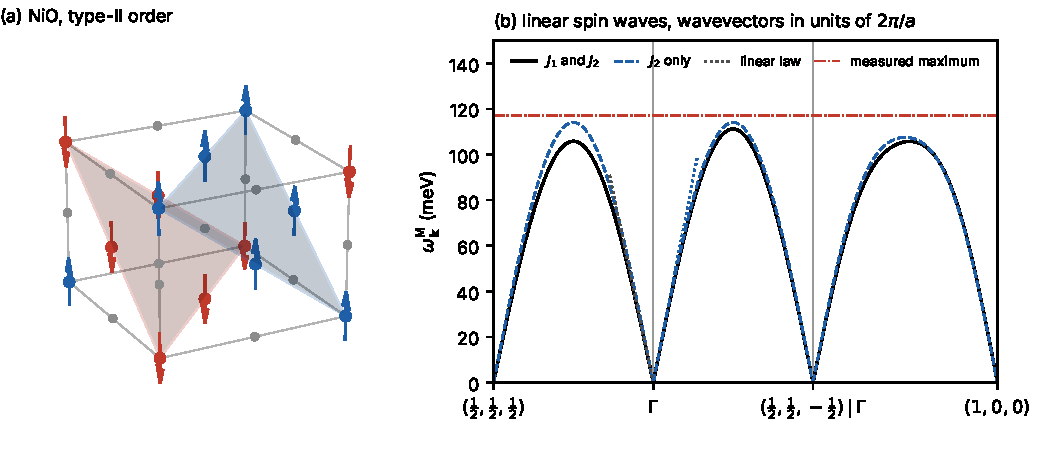
\includegraphics[width=\linewidth]{figures/ch07/fig7_1.pdf}
  \caption{Magnetic order and spin waves of NiO. (a) Conventional cubic cell of the rock-salt structure: nickel ions (colored) on the fcc sites, oxygen ions (gray) between them. In the type-II order the spins of each $(111)$ plane are parallel and alternate in sign from plane to plane; two of these planes are shaded. The arrows show only the sign of each moment; in NiO the moments lie within the planes, along a direction set by the weak anisotropy. (b) Magnon energies $\omega^{\mathrm{M}}_{\vect{k}}$ (meV) from linear spin-wave theory, \cref{eq:7.1-afm}, along three lines from the zone center $\Gamma$, with wavevectors in units of $2\pi/a$ and $a = \SI{4.17}{\angstrom}$. Model: undistorted fcc lattice, Heisenberg exchange with $J_1 = -\SI{1.37}{meV}$ and $J_2 = \SI{19.01}{meV}$ (each pair counted once, positive antiferromagnetic) measured by neutron scattering, $|\vect{S}| = 1$, no anisotropy. Solid: $J_1$ and $J_2$; dashed: $J_2$ alone, \cref{eq:7.1-J2}. Dotted: the linear laws $2\sqrt3(J_1 + J_2)|\vect{S}|ak$ along $[111]$, and $2\sqrt3J_2|\vect{S}|ak$ for $J_2$ alone. Dash-dotted: the measured maximum, ${\sim}\SI{117}{meV}$. The point $(\frac12,\frac12,\frac12)$, along the stacking direction of the planes, is equivalent to $\Gamma$ in the magnetic structure, and the energy returns to zero there. The zeros at $(\frac12,\frac12,-\frac12)$ and $(1,0,0)$ are soft points of the undistorted model; in real NiO the small rhombohedral distortion lifts them to a few meV. The largest energy in the zone, $|\vect{S}|(6J_2 - 3J_1) = \SI{118.2}{meV}$, lies off these lines.}
  \label{fig:7-nio}
\end{figure}

\begin{workedexample}{The magnon velocity of NiO}\label{we:7-nio}
With the exchange constants \cref{eq:7.1-NiO}, $|\vect{S}| = 1$ for Ni$^{2+}$, and the measured lattice constant $a = \SI{4.17}{\angstrom}$ as tabulated by Fischer et al.~\cite[Table~I]{fischer2009exchange}, \cref{eq:7.1-J2} gives the magnon velocity for $J_2$ alone
\begin{equation*}
  2\sqrt3\,J_2|\vect{S}|\,a = 2\sqrt3\times\SI{19.01}{meV}\times\SI{4.17}{\angstrom} = \SI{274.6}{meV.\angstrom} .
\end{equation*}
Dividing by $\hbar c = \SI{1973.27}{eV.\angstrom}$ turns this velocity into $1.39\times10^{-4}$ in natural units, or \SI{41.7}{km/s}. The nearest-neighbor exchange modifies the velocity. Along $[111]$, the direction normal to the ferromagnetic planes, the 6 parallel neighbors lie in a plane perpendicular to $\vect{k}$ and drop out of \cref{eq:D.19-linear}. Each of the 6 antiparallel ones has $(\vect{k}\cdot\vect{\delta})^2 = a^2k^2/3$, the same as each next-nearest neighbor contributes on average, and $J^{\mathrm{ex}}_{\mathrm{AB}}(0) = 6(J_1 + J_2)$. The bracket of \cref{eq:D.19-linear} is $2a^2k^2(J_1 + J_2)$, and
\begin{equation*}
  \omega^{\mathrm{M}}_{\vect{k}} \simeq 2\sqrt3\,(J_1 + J_2)|\vect{S}|\,ak = \SI{254.8}{meV.\angstrom}\times k \qquad (\vect{k} \parallel [111]) .
\end{equation*}
In other directions the parallel bonds no longer drop out, and evaluating \cref{eq:7.1-afm} numerically at small $k$ gives slopes between 255 and \SI{269}{meV.\angstrom}. The measured initial slope is ${\sim}\SI{250}{meV.\angstrom}$.

The largest magnon energy follows from a bound. With $J_1 < 0$, the in-plane sum $J^{\mathrm{ex}}_{\mathrm{AA}}(\vect{k}) = J_1\sum_{\vect{\delta}}\cos\vect{k}\cdot\vect{\delta}$ over the 6 parallel neighbors is largest when the cosines sum to their minimum, $-3$, the value of a triangular lattice at the corner of its zone. Then $A_{\vect{k}} \le J^{\mathrm{ex}}_{\mathrm{AB}}(0) - J^{\mathrm{ex}}_{\mathrm{AA}}(0) - 3J_1 = 6J_2 - 3J_1$, and $\omega^{\mathrm{M}}_{\vect{k}} \le |\vect{S}|A_{\vect{k}}$ with equality where $B_{\vect{k}} = 0$. The cosine minimum and the condition $B_{\vect{k}} = 0$ hold at the same $\vect{k}$, where $\omega^{\mathrm{M}}_{\mathrm{max}} = |\vect{S}|(6J_2 - 3J_1) = \SI{118.2}{meV}$, against $6J_2|\vect{S}| = \SI{114.1}{meV}$ for $J_2$ alone and a measured maximum of ${\sim}\SI{117}{meV}$. Linear spin-wave theory with two exchange constants thus reproduces both ends of the measured spectrum to a few percent. The agreement is partly by construction, since the exchange constants were fitted to the same data, and it does not test the $1/|\vect{S}|$ corrections, which a fit absorbs into $J_1$ and $J_2$.

The magnon velocity, $1.39\times10^{-4}$, is 19 times smaller than the fastest dark-matter speed in the laboratory, $v_{\mathrm{max}} = 2.650\times10^{-3}$ (\cref{sec:1.3}), and five times larger than the longitudinal sound speed of silicon, \SI{8.43}{km/s} along $[100]$ (\cref{app:C.18}). A dark-matter particle moves faster than the magnons it can emit. Emitting a magnon near the zone center is kinematically allowed in the same way as emitting an acoustic phonon, and at the same momentum transfer magnon emission deposits about five times more energy than phonon emission.
\end{workedexample}

\subsection{Spin-density response}

A probe that couples to the spin of the electron, such as a slow neutron or a dark-matter particle with a spin-dependent interaction, couples to the \emph{electron spin density}
\begin{equation}
  \vect{s}_e(\vect{q}) = \sum_i\ee^{\ii\vect{q}\cdot\vect{r}_i}\,\frac{\vect{\sigma}_i}{2} ,
  \label{eq:7.1-se}
\end{equation}
the spin analog of the density $n_e(\vect{q})$ of \cref{sec:2.3}, with the Pauli matrices $\vect{\sigma}_i$ of electron $i$. Like $n_e(\vect{q})$, the spin density $\vect{s}_e(\vect{q})$ adds the momentum $\vect{q}$ to the target. For dark matter of spin $\frac12$ with a spin-dependent coupling, the interaction takes the form $-\sum_a\hat O_{\chi a}(\vect{q})\,s_{e,a}(\vect{q})$~\cite[Eq.~(4)]{trickle2020detecting}, with an operator $\hat O_{\chi a}$ that acts on the spin of the dark-matter particle; \cref{sec:8.1} lists and derives these operators. The three components $s_{e,a}(\vect{q})$ are then target operators $O_a$ of the response matrix $S_{ab}$ of \cref{eq:4.2-Sab}, as the density was for a charge coupling.

In a magnetic insulator the spin density is localized on the ions. The filled shells carry no spin, and the unpaired electrons of ion $j$ occupy an open shell whose spin, at low energy, is $\vect{S}_j$. Within the ground multiplet of the ion every vector operator is proportional to $\vect{S}_j$, by the Wigner--Eckart theorem: the matrix elements of any vector operator within a multiplet of fixed total spin are those of the spin itself times one constant. The spin density near ion $j$ is therefore $\vect{S}_j\,\varrho_{\mathrm{s}}(\vect{r} - \vect{R}_j)$, with $\varrho_{\mathrm{s}}$ the normalized density of the unpaired electrons. The Fourier transform of the spin density is
\begin{equation}
  \vect{s}_e(\vect{q}) = F^{\mathrm{mag}}(q)\sum_j\ee^{\ii\vect{q}\cdot\vect{R}_j}\,\vect{S}_j, \qquad
  F^{\mathrm{mag}}(q) = \int\dd^3r\,\ee^{\ii\vect{q}\cdot\vect{r}}\,\varrho_{\mathrm{s}}(\vect{r}) ,
  \label{eq:7.1-Fmag}
\end{equation}
where $F^{\mathrm{mag}}(q)$, the \emph{magnetic form factor} of the ion, is spherically averaged and normalized to $F^{\mathrm{mag}}(0) = 1$. It is the spin analog of the atomic form factor of \cref{sec:2.2}. For a $3d$ shell it stays close to one up to the inverse shell radius, a few \si{\angstrom^{-1}} or several keV (\cref{app:C.19}), above most momentum transfers of sub-MeV dark matter. \Cref{app:C.19} adds the orbital moment of shells that have one and derives the neutron cross-section, which measures the same $S_{ab}$. \Cref{eq:7.1-Fmag} reduces the response of the electrons to the response of the ionic spins, a quantity that linear spin-wave theory supplies.

For the ferromagnet, at zero temperature, the transverse spin operators create single magnons. Define $S^\pm(\vect{q}) = \sum_j\ee^{\ii\vect{q}\cdot\vect{R}_j}S^\pm_j$. At linear order $S^-_j \simeq (2|\vect{S}|)^{1/2}d^\dagger_j$, and with $d^\dagger_j = N^{-1/2}\sum_{\vect{k}}\ee^{-\ii\vect{k}\cdot\vect{R}_j}a^\dagger_{\vect{k}}$ and the lattice sum \cref{eq:3.1-latticesum},
\begin{equation*}
  S^-(\vect{q}) \simeq (2|\vect{S}|N)^{1/2}\,a^\dagger_{\vect{q}_r} ,
\end{equation*}
where $\vect{q} = \vect{q}_r + \vect{G}_{\vect{q}}$ is the split of \cref{eq:3.1-qsplit} into a wavevector in the zone and a reciprocal-lattice vector. Crystal momentum is conserved: the magnon carries $\vect{q}_r$, and the lattice takes $\vect{G}_{\vect{q}}$. The operator $S^+(\vect{q})$ annihilates the ground state, which is fully polarized, and $S^z$ is quadratic in the bosons and creates no single magnon. With $s_{e,x} = F^{\mathrm{mag}}(S^+ + S^-)/2$ and $s_{e,y} = F^{\mathrm{mag}}(S^+ - S^-)/2\ii$, the one-magnon matrix elements are $\langle\vect{q}_r|s_{e,x}|0\rangle = F^{\mathrm{mag}}(2|\vect{S}|N)^{1/2}/2$ and $\langle\vect{q}_r|s_{e,y}|0\rangle = \ii F^{\mathrm{mag}}(2|\vect{S}|N)^{1/2}/2$. Inserting them into \cref{eq:4.2-Sab} with $\Vol = N\Omega$, where $\Omega$ is the volume per magnetic ion, gives:
\begin{keyresult}[One-magnon spin response of a ferromagnet]
\begin{equation}
  S_{ab}(\vect{q},\omega) = \frac{\pi|\vect{S}|}{\Omega}\,|F^{\mathrm{mag}}(q)|^2\,\bigl(\delta_{ab} - \hat z_a\hat z_b + \ii\epsilon_{abc}\hat z_c\bigr)\,\delta\bigl(\omega - \omega^{\mathrm{M}}_{\vect{q}_r}\bigr) ,
  \label{eq:7.1-Sfm}
\end{equation}
for $T = 0$, $\omega > 0$, and spins ordered along $\hat{\vect{z}}$, with $a, b$ the Cartesian components of $\vect{s}_e$.
\end{keyresult}
The matrix in brackets has the eigenvalues 2, for the circular combination $s_{e,x} - \ii s_{e,y}$ that lowers the spin, and 0 for the other two: \cref{eq:7.1-Sfm} is Hermitian and positive semidefinite, as \cref{eq:4.2-positivity} requires. A ferromagnet absorbs only the sense of rotation in which its spins precess, and this sense of rotation is the polarization vector $(|\vect{S}|/2)^{1/2}(1, \ii, 0)$ of Ref.~\cite[Eq.~(6)]{trickle2020detecting}. Apart from $|F^{\mathrm{mag}}|^2$ the one-magnon weight does not depend on $\vect{q}$. Through the fluctuation--dissipation theorem \cref{eq:4.2-fdt}, the same delta function is a pole of the transverse spin response $R_{ab}$, the susceptibility that magnetic resonance and neutron scattering measure.

In the antiferromagnet a transverse spin operator again creates one magnon, now with the amplitudes of \cref{eq:7.1-bogo}. The part of $S^+(\vect{k})$ on A is to linear order $S^+_{\mathrm{A}}(\vect{k}) \equiv \sum_{i\in\mathrm{A}}\ee^{\ii\vect{k}\cdot\vect{R}_i}S^+_i = (2|\vect{S}|N_{\mathrm{s}})^{1/2}d_{\mathrm{A},-\vect{k}}$, by the lattice sum $\sum_i\ee^{\ii(\vect{k}+\vect{k}')\cdot\vect{R}_i} = N_{\mathrm{s}}\delta_{\vect{k},-\vect{k}'}$. Inverting \cref{eq:7.1-bogo} as in \cref{app:C.7} gives
\begin{equation}
  d_{\mathrm{A}\vect{k}} = u^{\mathrm{M}}_{\vect{k}}\,a_{\vect{k}1} - v^{\mathrm{M}}_{\vect{k}}\,a^\dagger_{\vect{k}2}, \qquad
  d_{\mathrm{B}\vect{k}} = u^{\mathrm{M}}_{\vect{k}}\,a_{\vect{k}2} - v^{\mathrm{M}}_{\vect{k}}\,a^\dagger_{\vect{k}1} .
  \label{eq:D.19-inverse}
\end{equation}
On B the raising operator is $S^+_j \simeq (2|\vect{S}|)^{1/2}d^\dagger_{\mathrm{B}j}$, and the same lattice sum turns $\sum_{j\in\mathrm{B}}\ee^{\ii\vect{k}\cdot\vect{R}_j}d^\dagger_{\mathrm{B}j}$ into $N_{\mathrm{s}}^{1/2}d^\dagger_{\mathrm{B},-\vect{k}}$. Since $A_{\vect{k}}$ and $B_{\vect{k}}$, and with them $u^{\mathrm{M}}_{\vect{k}}$ and $v^{\mathrm{M}}_{\vect{k}}$, are even in $\vect{k}$, the sum of the contributions of both sublattices at small $\vect{k}$ is $S^+(\vect{k}) \simeq (2|\vect{S}|N_{\mathrm{s}})^{1/2}(d_{\mathrm{A},-\vect{k}} + d^\dagger_{\mathrm{B},-\vect{k}}) = (2|\vect{S}|N_{\mathrm{s}})^{1/2}(u^{\mathrm{M}}_{\vect{k}} - v^{\mathrm{M}}_{\vect{k}})(a_{-\vect{k}1} + a^\dagger_{-\vect{k}2})$. Near the ordering wavevector, where the two sublattices enter with opposite phases, the one-magnon amplitude is $(2|\vect{S}|N_{\mathrm{s}})^{1/2}(u^{\mathrm{M}}_{\vect{k}} + v^{\mathrm{M}}_{\vect{k}})$. From the expressions of $\cosh2\theta_{\vect{k}}$ and $\sinh2\theta_{\vect{k}}$ in \cref{app:C.7},
\begin{equation}
  \bigl(u^{\mathrm{M}}_{\vect{k}} \mp v^{\mathrm{M}}_{\vect{k}}\bigr)^2 = \frac{A_{\vect{k}} \mp B_{\vect{k}}}{(A_{\vect{k}}^2 - B_{\vect{k}}^2)^{1/2}} = \frac{|\vect{S}|(A_{\vect{k}} \mp B_{\vect{k}})}{\omega^{\mathrm{M}}_{\vect{k}}} .
  \label{eq:7.1-weights}
\end{equation}
Near $\Gamma$, $A_{\vect{k}} - B_{\vect{k}} \propto k^2$ while $\omega^{\mathrm{M}}_{\vect{k}} \propto k$, so the weight near $\Gamma$ vanishes linearly in $k$: a uniform field cannot tilt two opposite sublattices without working against the exchange field. Near the ordering wavevector the weight grows as the inverse distance from that wavevector. Unlike the ferromagnet, the antiferromagnet thus distributes its one-magnon weight unevenly: at the same $\vect{k}$ the weights near $\Gamma$ and near the ordering wavevector differ by the factor $(A_{\vect{k}} + B_{\vect{k}})/(A_{\vect{k}} - B_{\vect{k}})$. Dark matter samples the suppressed weight near $\Gamma$ unless its momentum transfer reaches the ordering wavevector, $(\pi/a)(1,1,1)$ in NiO, of length $\sqrt3\pi/a = \SI{1.30}{\angstrom^{-1}} = \SI{2.6}{keV}$. Since $q \le 2\mchi v_{\mathrm{max}}$, reaching the ordering wavevector takes $\mchi \gtrsim \SI{0.5}{MeV}$. The longitudinal component $S^z$ creates magnons in pairs.
